\documentclass[usenames,dvipsnames,tikz]{standalone}
\usepackage{amsmath,amssymb}
\usepackage{xcolor}
\colorlet{tBlue}{RoyalBlue!35!Cerulean}
\colorlet{tRed}{Red}
\usepackage{tikz}
\usepackage{standalone}
\begin{document}
	
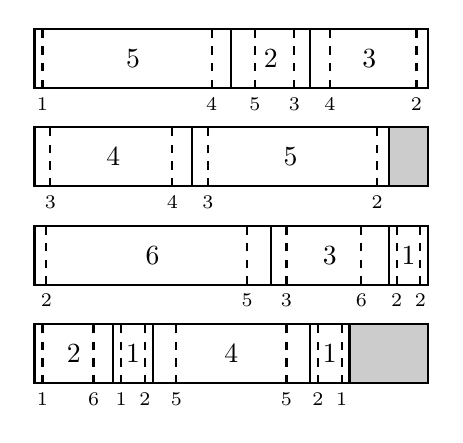
\begin{tikzpicture}
%\draw [help lines] (-1,-2) grid (6,5);
% 1=0.1, 2=0.15, 3=0.2, 4=0.25, 5=0.3
%A=2,(2-4), B=2,(4-5), C=3,(1-3), D=3,(2-3), E=3,(4-4), F=4(1-3), G=4(1-5), H=5(1-2)

\draw [thick] (0,0) rectangle (5,0.75);
\draw [thick] (0,1.25) rectangle (5,2);
\draw [thick] (0,2.5) rectangle (5,3.25);
\draw [thick] (0,3.75) rectangle (5,4.5);

% Bottom row, 2, 1, 4, 1 (1-6, 1-2, 5-5, 2-1)
\draw [thick] (1,0) -- (1,0.75);
\draw [thick] (1.5,0) -- (1.5,0.75);
\draw [thick] (3.5,0) -- (3.5,0.75);
\draw [thick] (4,0) -- (4,0.75);
\filldraw[fill=black!20!white, draw=black, thick] (4,0) rectangle (5,0.75);
\draw [thick, dashed] (0.1,0) -- (0.1,0.75);
\draw [thick, dashed] (0.75,0) -- (0.75,0.75);
\draw [thick, dashed] (1.1,0) -- (1.1,0.75);
\draw [thick, dashed] (1.4,0) -- (1.4,0.75);
\draw [thick, dashed] (1.8,0) -- (1.8,0.75);
\draw [thick, dashed] (3.2,0) -- (3.2,0.75);
\draw [thick, dashed] (3.6,0) -- (3.6,0.75);
\draw [thick, dashed] (3.9,0) -- (3.9,0.75);
\node [below] at (0.1,0) {\scriptsize{1}};
\node [below] at (0.75,0) {\scriptsize{6}};
\node [below] at (1.1,0) {\scriptsize{1}};
\node [below] at (1.4,0) {\scriptsize{2}};
\node [below] at (1.8,0) {\scriptsize{5}};
\node [below] at (3.2,0) {\scriptsize{5}};
\node [below] at (3.6,0) {\scriptsize{2}};
\node [below] at (3.9,0) {\scriptsize{1}};
\node at (0.5,0.375) {2};
\node at (1.25,0.375) {1};
\node at (2.5,0.375) {4};
\node at (3.75,0.375) {1};

% Second from bottom row, 6, 3, 1 (2-5, 3-6, 2-2)
\draw [thick] (3,1.25) -- (3,2);
\draw [thick] (4.5,1.25) -- (4.5,2);
\draw [thick, dashed] (0.15,1.25) -- (0.15,2);
\draw [thick, dashed] (2.7,1.25) -- (2.7,2);
\draw [thick, dashed] (3.2,1.25) -- (3.2,2);
\draw [thick, dashed] (4.15,1.25) -- (4.15,2);
\draw [thick, dashed] (4.6,1.25) -- (4.6,2);
\draw [thick, dashed] (4.9,1.25) -- (4.9,2);
\node [below] at (0.15,1.25) {\scriptsize{2}};
\node [below] at (2.7,1.25) {\scriptsize{5}};
\node [below] at (3.2,1.25) {\scriptsize{3}};
\node [below] at (4.15,1.25) {\scriptsize{6}};
\node [below] at (4.6,1.25) {\scriptsize{2}};
\node [below] at (4.9,1.25) {\scriptsize{2}};
\node at (1.5,1.625) {6};
\node at (3.75,1.625) {3};
\node at (4.75,1.625) {1};

% Second from top row, 4, 5 (3-4, 3-2)
\draw [thick] (2,2.5) -- (2,3.25);
\draw [thick] (4.5,2.5) -- (4.5,3.25);
\filldraw[fill=black!20!white, draw=black, thick] (4.5,2.5) rectangle (5,3.25);
\draw [thick, dashed] (0.2,2.5) -- (0.2,3.25);
\draw [thick, dashed] (1.75,2.5) -- (1.75,3.25);
\draw [thick, dashed] (2.2,2.5) -- (2.2,3.25);
\draw [thick, dashed] (4.35,2.5) -- (4.35,3.25);
\node [below] at (0.2,2.5) {\scriptsize{3}};
\node [below] at (1.75,2.5) {\scriptsize{4}};
\node [below] at (2.2,2.5) {\scriptsize{3}};
\node [below] at (4.35,2.5) {\scriptsize{2}};
\node at (1,2.875) {4};
\node at (3.25,2.875) {5};

% Top row, 5, 2, 3 (1-4, 5-3, 4-2) 
\draw [thick] (2.5,3.75) -- (2.5,4.5);
\draw [thick] (3.5,3.75) -- (3.5,4.5);
\draw [thick, dashed] (0.1,3.75) -- (0.1,4.5);
\draw [thick, dashed] (2.25,3.75) -- (2.25,4.5);
\draw [thick, dashed] (2.8,3.75) -- (2.8,4.5);
\draw [thick, dashed] (3.3,3.75) -- (3.3,4.5);
\draw [thick, dashed] (3.75,3.75) -- (3.75,4.5);
\draw [thick, dashed] (4.85,3.75) -- (4.85,4.5);
\node [below] at (0.1,3.75) {\scriptsize{1}};
\node [below] at (2.25,3.75) {\scriptsize{4}};
\node [below] at (2.8,3.75) {\scriptsize{5}};
\node [below] at (3.3,3.75) {\scriptsize{3}};
\node [below] at (3.75,3.75) {\scriptsize{4}};
\node [below] at (4.85,3.75) {\scriptsize{2}};
\node at (1.25,4.125) {5};
\node at (3,4.125) {2};
\node at (4.25,4.125) {3};

\end{tikzpicture}

\end{document}